\documentclass{beamer}
\usetheme{Boadilla}
\usepackage{booktabs}
\usefonttheme{serif}
\subtitle{Using Beamer}
\usepackage{pgffor}

\title{ \textbf{Stepscan Project}}
\subtitle{Results of Worksheet 1-3}
\date{\today}
\author{Saeed Kazemi}
\institute{ University of New Brunswick}
\usepackage{caption}

\begin{document}


%%%%%%%%%%%%%%%%%%%%%%%%%%%%%%%%%%%%%%%%%%%
%%%%%%%%%%%%%%%%%%%%%%%%%%%%%%%%%%%%%%%%%%%
\begin{frame}
\titlepage
\end{frame}


%%%%%%%%%%%%%%%%%%%%%%%%%%%%%%%%%%%%%%%%%%%
%%%%%%%%%%%%%%%%%%%%%%%%%%%%%%%%%%%%%%%%%%%
\begin{frame}
\frametitle{Outline}
\tableofcontents
\end{frame}


%%%%%%%%%%%%%%%%%%%%%%%%%%%%%%%%%%%%%%%%%%%
%%%%%%%%%%%%%%%%%%%%%%%%%%%%%%%%%%%%%%%%%%%
\foreach \n in {Score Matrix}{
\section{\n}
\def \variable {Correlation}
\foreach \t in {Euclidean Distance, Correlation}{

\begin{frame}
\frametitle{\t}
\tiny
\begin{table}
\centering
\captionsetup{labelformat=empty}
\caption{\small The accuracy and ERR of \t.}
\label{tab:parameters condition}
\input{tables/\t.tex}
\end{table}
\end{frame}
}

\begin{frame}
\centering
\frametitle{The ROC curve}
\includegraphics[scale=0.3]{Manuscripts/src/figures/\variable_ROC.png}
\end{frame}
}


%%%%%%%%%%%%%%%%%%%%%%%%%%%%%%%%%%%%%%%%%%%
%%%%%%%%%%%%%%%%%%%%%%%%%%%%%%%%%%%%%%%%%%%
\foreach \n in {Model type}{
\section{\n}
\def \variable {Median}
\foreach \t in {Minimum, Median, Average}{

\begin{frame}
\frametitle{\t \ Model}
\tiny
\begin{table}
\centering
\captionsetup{labelformat=empty}
\caption{\small The accuracy and ERR of \t \ model.}
\label{tab:parameters condition}
\input{tables/\t.tex}
\end{table}
\end{frame}
}

\begin{frame}
\centering
\frametitle{The ROC curve}
\includegraphics[scale=0.3]{Manuscripts/src/figures/\variable_ROC.png}
\end{frame}
}


%%%%%%%%%%%%%%%%%%%%%%%%%%%%%%%%%%%%%%%%%%%
%%%%%%%%%%%%%%%%%%%%%%%%%%%%%%%%%%%%%%%%%%%
\foreach \n in {PCA}{
\section{\n}
\def \variable {PCA} %PCA
\foreach \t in {All Data, Keeping 95 percent of variance}{

\begin{frame}
\frametitle{\t}
\tiny
\begin{table}
\centering
\captionsetup{labelformat=empty}
\caption{\small The accuracy and ERR of \t.}
\label{tab:parameters condition}
\input{tables/\t.tex}
\end{table}
\end{frame}
}

\begin{frame}
\centering
\frametitle{The ROC curve}
\includegraphics[scale=0.3]{Manuscripts/src/figures/\variable_ROC.png}
\end{frame}
}

%%%%%%%%%%%%%%%%%%%%%%%%%%%%%%%%%%%%%%%%%%%
%%%%%%%%%%%%%%%%%%%%%%%%%%%%%%%%%%%%%%%%%%%
\foreach \n in {Test size}{
\section{\n}
\def \variable {testsize}%testsize
\foreach \t in {20 percent, 35 percent, 50 percent}{

\begin{frame}
\frametitle{\t \ \n}
\tiny
\begin{table}
\centering
\caption{\small The accuracy and ERR of \t \  \n.}
\input{tables/\t.tex}
\end{table}
\end{frame}
}

\begin{frame}
\centering
\frametitle{The ROC curve}
\includegraphics[scale=0.3]{Manuscripts/src/figures/\variable_ROC.png}
\end{frame}
}


%%%%%%%%%%%%%%%%%%%%%%%%%%%%%%%%%%%%%%%%%%%
%%%%%%%%%%%%%%%%%%%%%%%%%%%%%%%%%%%%%%%%%%%
\foreach \n in {Normalization algorithm}{
\section{\n}
\def \variable {MinMax}%MinMax
\foreach \t in {Z-score algorithm, MinMax algorithm, None}{

\begin{frame}
\frametitle{\t}
\tiny
\begin{table}
\centering
\captionsetup{labelformat=empty}
\caption{\small The accuracy and ERR of \t.}
\label{tab:parameters condition}
\input{tables/\t.tex}
\end{table}
\end{frame}
}

\begin{frame}
\centering
\frametitle{The ROC curve}
\includegraphics[scale=0.3]{Manuscripts/src/figures/\variable_ROC.png}
\end{frame}
}



%%%%%%%%%%%%%%%%%%%%%%%%%%%%%%%%%%%%%%%%%%%
%%%%%%%%%%%%%%%%%%%%%%%%%%%%%%%%%%%%%%%%%%%
\foreach \n in {COP features}{
\section{\n}
\def \variable {feat}%feat
\foreach \t in {All features, Only MDIST features, Only RDIST features, Only TOTEX features, Only MVELO features, Only RANGE features, Only AREAXX features, Only MFREQ features, Only FDPD features, Only FDCX features}{  

\begin{frame}
\frametitle{\t}
\tiny
\begin{table}
\centering
\captionsetup{labelformat=empty}
\caption{\tiny The accuracy and ERR of \t.}
\label{tab:parameters condition}
\input{tables/\t.tex}
\end{table}
\end{frame}
}

\begin{frame}
\centering
\frametitle{The ROC curve}
\includegraphics[scale=0.3]{Manuscripts/src/figures/\variable_ROC.png}
\end{frame}
}


%%%%%%%%%%%%%%%%%%%%%%%%%%%%%%%%%%%%%%%%%%%
%%%%%%%%%%%%%%%%%%%%%%%%%%%%%%%%%%%%%%%%%%%
\section{The top-10 best and worst features}

\begin{frame}[shrink=10]
\frametitle{The top-10 best features for the left foot.}
\tiny
\begin{table}
\begin{adjustbox}
\centering
\caption{\small The top-10 best features for the left foot.}
\begin{tabular}{lllrllrrr}
\toprule
{} &  Mode & Model\_Type &  TestSize &     Norm & Features\_Set &   PCA &  Acc\_Left &  EER\_Left \\
index &       &            &           &          &              &       &           &           \\
\midrule
832   &  corr &     median &       0.2 &  z-score &       AREAXX &  0.95 &     98.96 &      0.05 \\
1012  &  corr &     median &       0.2 &   minmax &       AREAXX &  0.95 &     98.96 &      0.05 \\
652   &  corr &     median &       0.2 &     None &       AREAXX &  0.95 &     98.96 &      0.05 \\
526   &  corr &     median &       0.2 &   minmax &         FDCX &  1.00 &     98.96 &      0.06 \\
688   &  corr &     median &       0.2 &     None &         FDPD &  0.95 &     98.96 &      0.06 \\
94    &  corr &     median &       0.2 &     None &        RANGE &  1.00 &     98.96 &      0.06 \\
1048  &  corr &     median &       0.2 &   minmax &         FDPD &  0.95 &     98.96 &      0.06 \\
454   &  corr &     median &       0.2 &   minmax &        RANGE &  1.00 &     98.96 &      0.06 \\
346   &  corr &     median &       0.2 &  z-score &         FDCX &  1.00 &     98.96 &      0.06 \\
868   &  corr &     median &       0.2 &  z-score &         FDPD &  0.95 &     98.96 &      0.07 \\
\bottomrule
\end{tabular}

\end{adjustbox}
\end{table}
\end{frame}

%%%%%%%%%%%%%%%%%%%%%%%%%%%%%%%%%%%%%%%%%%%
%%%%%%%%%%%%%%%%%%%%%%%%%%%%%%%%%%%%%%%%%%%
\begin{frame}[shrink=10]
\frametitle{The top-10 best features for the right foot.}
\tiny
\begin{table}
\begin{adjustbox}
\centering
\caption{\small The top-10 best features for the right foot.}
\begin{tabular}{lllrllrrr}
\toprule
{} &  Mode & Model\_Type &  Test\_Size & Normalizition & Features\_Set &   PCA &  Mean\_Accuracy\_Right &  Mean\_EER\_Right \\
index &       &            &            &               &              &       &                      &                 \\
\midrule
346   &  corr &     median &        0.2 &       z-score &         FDCX &  1.00 &                98.96 &            0.05 \\
94    &  corr &     median &        0.2 &          None &        RANGE &  1.00 &                98.96 &            0.05 \\
832   &  corr &     median &        0.2 &       z-score &       AREAXX &  0.95 &                98.96 &            0.05 \\
652   &  corr &     median &        0.2 &          None &       AREAXX &  0.95 &                98.96 &            0.05 \\
1012  &  corr &     median &        0.2 &        minmax &       AREAXX &  0.95 &                98.96 &            0.05 \\
526   &  corr &     median &        0.2 &        minmax &         FDCX &  1.00 &                98.96 &            0.05 \\
688   &  corr &     median &        0.2 &          None &         FDPD &  0.95 &                98.96 &            0.05 \\
1048  &  corr &     median &        0.2 &        minmax &         FDPD &  0.95 &                98.96 &            0.06 \\
454   &  corr &     median &        0.2 &        minmax &        RANGE &  1.00 &                98.96 &            0.06 \\
868   &  corr &     median &        0.2 &       z-score &         FDPD &  0.95 &                98.96 &            0.06 \\
\bottomrule
\end{tabular}

\end{adjustbox}
\end{table}
\end{frame}

%%%%%%%%%%%%%%%%%%%%%%%%%%%%%%%%%%%%%%%%%%%
%%%%%%%%%%%%%%%%%%%%%%%%%%%%%%%%%%%%%%%%%%%
\begin{frame}[shrink=10]
\frametitle{The top-10 worst features for the left foot.}
\tiny
\begin{table}
\begin{adjustbox}
\centering
\caption{\small The top-10 worst features for the left foot.}
\begin{tabular}{lllrllrrr}
\toprule
{} &  Mode & Model\_Type &  Test\_Size & Normalizition & Features\_Set &   PCA &  Mean\_Accuracy\_Left &  Mean\_EER\_Left \\
index &       &            &            &               &              &       &                     &                \\
\midrule
655   &  corr &    average &        0.2 &          None &       AREAXX &  0.95 &                1.04 &           0.67 \\
529   &  corr &    average &        0.2 &        minmax &         FDCX &  1.00 &                1.04 &           0.66 \\
1015  &  corr &    average &        0.2 &        minmax &       AREAXX &  0.95 &                1.04 &           0.66 \\
835   &  corr &    average &        0.2 &       z-score &       AREAXX &  0.95 &                1.04 &           0.66 \\
691   &  corr &    average &        0.2 &          None &         FDPD &  0.95 &                1.04 &           0.66 \\
1051  &  corr &    average &        0.2 &        minmax &         FDPD &  0.95 &                1.04 &           0.65 \\
871   &  corr &    average &        0.2 &       z-score &         FDPD &  0.95 &                1.04 &           0.64 \\
457   &  corr &    average &        0.2 &        minmax &        RANGE &  1.00 &                1.04 &           0.64 \\
349   &  corr &    average &        0.2 &       z-score &         FDCX &  1.00 &                1.04 &           0.62 \\
277   &  corr &    average &        0.2 &       z-score &        RANGE &  1.00 &                1.04 &           0.62 \\
\bottomrule
\end{tabular}

\end{adjustbox}
\end{table}
\end{frame}

%%%%%%%%%%%%%%%%%%%%%%%%%%%%%%%%%%%%%%%%%%%
%%%%%%%%%%%%%%%%%%%%%%%%%%%%%%%%%%%%%%%%%%%
\begin{frame}[shrink=10]
\frametitle{The top-10 worst features for the right foot.}
\tiny
\begin{table}
\begin{adjustbox}
\centering
\caption{\small The top-10 worst features for the right foot.}
\begin{tabular}{lllrllrrr}
\toprule
{} &  Mode & Model\_Type &  TestSize &     Norm & Features\_Set &   PCA &  Acc\_Right &  EER\_Right \\
index &       &            &           &          &              &       &            &            \\
\midrule
529   &  corr &    average &       0.2 &   minmax &         FDCX &  1.00 &       1.04 &       0.67 \\
655   &  corr &    average &       0.2 &     None &       AREAXX &  0.95 &       1.04 &       0.67 \\
1015  &  corr &    average &       0.2 &   minmax &       AREAXX &  0.95 &       1.04 &       0.66 \\
835   &  corr &    average &       0.2 &  z-score &       AREAXX &  0.95 &       1.04 &       0.66 \\
691   &  corr &    average &       0.2 &     None &         FDPD &  0.95 &       1.04 &       0.65 \\
871   &  corr &    average &       0.2 &  z-score &         FDPD &  0.95 &       1.04 &       0.65 \\
1051  &  corr &    average &       0.2 &   minmax &         FDPD &  0.95 &       1.04 &       0.65 \\
349   &  corr &    average &       0.2 &  z-score &         FDCX &  1.00 &       1.04 &       0.63 \\
457   &  corr &    average &       0.2 &   minmax &        RANGE &  1.00 &       1.04 &       0.63 \\
169   &  corr &    average &       0.2 &     None &         FDCX &  1.00 &       1.04 &       0.63 \\
\bottomrule
\end{tabular}

\end{adjustbox}
\end{table}
\end{frame}


%%%%%%%%%%%%%%%%%%%%%%%%%%%%%%%%%%%%%%%%%%%
%%%%%%%%%%%%%%%%%%%%%%%%%%%%%%%%%%%%%%%%%%%
\section{Feature Selection}
\begin{frame}[shrink=10]
\frametitle{The top-10 best features based on feature selection algorithm.}
\tiny
\begin{table}
\begin{adjustbox}
\centering
\caption{\small The top-10 best features based on feature selection algorithm.}
\begin{tabular}{llllll}
\toprule
{} &     D-prime &     F-ratio &    mRMR-Dif &      mRMR-Q &  Redundancy \\
\midrule
0 &  feature\_20 &   feature\_0 &  feature\_20 &  feature\_20 &   feature\_3 \\
1 &  feature\_16 &   feature\_7 &  feature\_25 &  feature\_25 &   feature\_9 \\
2 &  feature\_25 &  feature\_10 &  feature\_16 &  feature\_18 &   feature\_6 \\
3 &   feature\_0 &  feature\_13 &  feature\_18 &  feature\_21 &  feature\_15 \\
4 &  feature\_18 &  feature\_12 &  feature\_21 &  feature\_16 &   feature\_4 \\
5 &  feature\_21 &   feature\_1 &   feature\_0 &  feature\_22 &   feature\_0 \\
6 &   feature\_1 &  feature\_16 &   feature\_2 &   feature\_2 &  feature\_13 \\
7 &   feature\_2 &  feature\_20 &   feature\_1 &   feature\_0 &  feature\_12 \\
8 &   feature\_7 &  feature\_18 &  feature\_24 &   feature\_1 &   feature\_7 \\
9 &  feature\_10 &  feature\_25 &   feature\_5 &  feature\_24 &  feature\_10 \\
\bottomrule
\end{tabular}

\end{adjustbox}
\end{table}
\end{frame}

%%%%%%%%%%%%%%%%%%%%%%%%%%%%%%%%%%%%%%%%%%%
%%%%%%%%%%%%%%%%%%%%%%%%%%%%%%%%%%%%%%%%%%%
\begin{frame}[shrink=10]
\frametitle{The top-10 worst features based on feature selection algorithm.}
\tiny
\begin{table}
\begin{adjustbox}
\centering
\caption{\small The top-10 worst features based on feature selection algorithm.}
\begin{tabular}{llllll}
\toprule
{} &     D-prime &     F-ratio &    mRMR-Dif &      mRMR-Q &  Redundancy \\
\midrule
16 &   feature\_8 &  feature\_22 &  feature\_11 &   feature\_8 &   feature\_2 \\
17 &  feature\_19 &   feature\_5 &   feature\_8 &  feature\_11 &  feature\_14 \\
18 &   feature\_4 &  feature\_19 &  feature\_23 &   feature\_3 &  feature\_21 \\
19 &  feature\_15 &  feature\_11 &   feature\_3 &   feature\_4 &  feature\_24 \\
20 &  feature\_14 &   feature\_8 &  feature\_14 &  feature\_14 &  feature\_18 \\
21 &  feature\_22 &  feature\_14 &   feature\_4 &  feature\_15 &  feature\_19 \\
22 &  feature\_17 &  feature\_17 &  feature\_15 &  feature\_23 &  feature\_25 \\
23 &  feature\_23 &   feature\_9 &  feature\_17 &  feature\_17 &  feature\_20 \\
24 &   feature\_9 &   feature\_6 &   feature\_6 &   feature\_6 &  feature\_23 \\
25 &   feature\_6 &  feature\_23 &   feature\_9 &   feature\_9 &  feature\_22 \\
\bottomrule
\end{tabular}

\end{adjustbox}
\end{table}
\end{frame}


%%%%%%%%%%%%%%%%%%%%%%%%%%%%%%%%%%%%%%%%%%%
%%%%%%%%%%%%%%%%%%%%%%%%%%%%%%%%%%%%%%%%%%%
\begin{frame}
\frametitle{The feature correlation plot.}
\centering
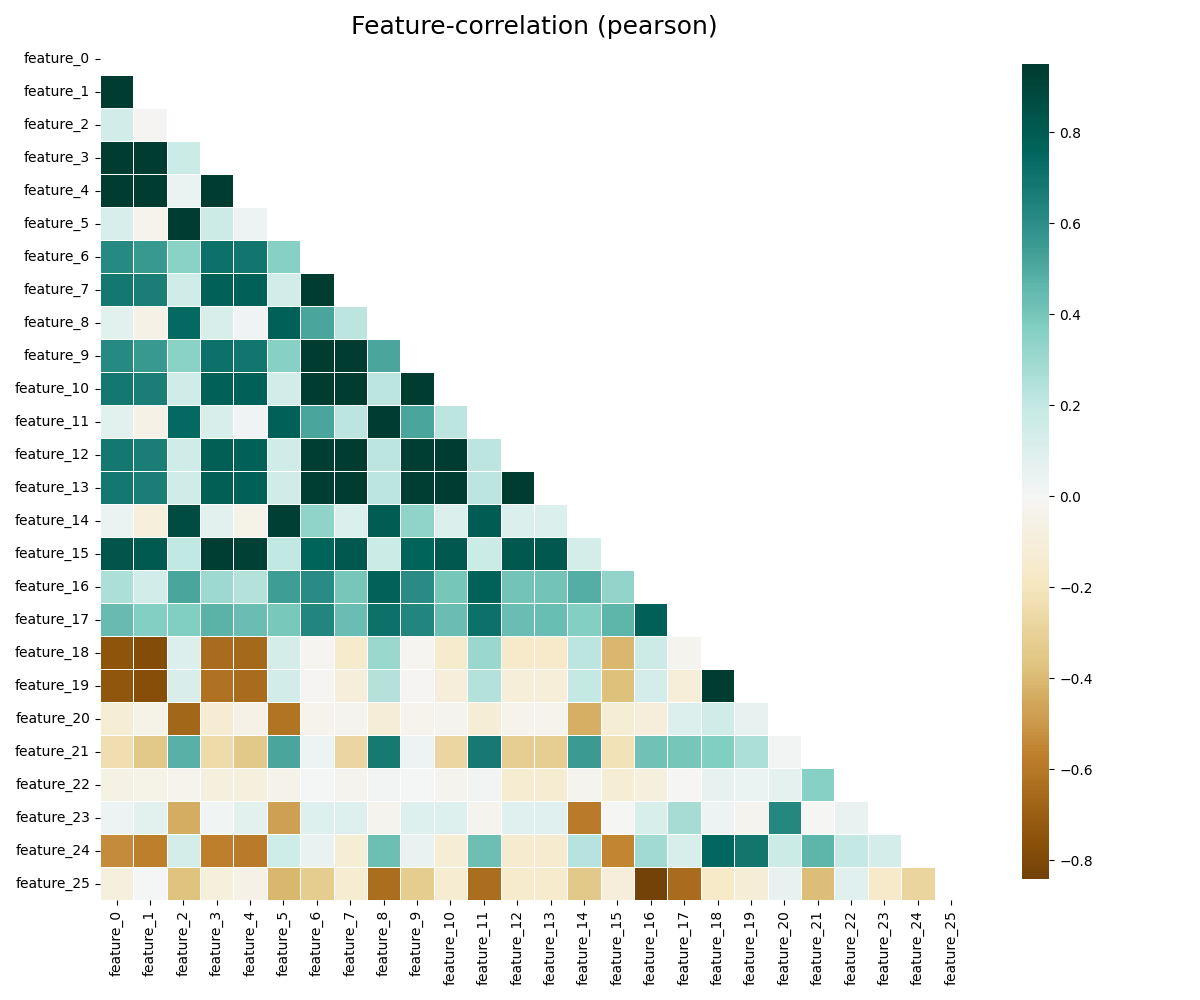
\includegraphics[scale=0.3]{Manuscripts/src/figures/corr_plot.png}
\end{frame}

%%%%%%%%%%%%%%%%%%%%%%%%%%%%%%%%%%%%%%%%%%%
%%%%%%%%%%%%%%%%%%%%%%%%%%%%%%%%%%%%%%%%%%%
\section{Summary}

\begin{frame}{Summary}

\begin{enumerate}[(I)]
\item Point A
\item Point B
\begin{enumerate}[(i)]
\item part 1
\item part 2
\end{enumerate}
\item Point C
\item Point D
\end{enumerate}
    
\end{frame}

%%%%%%%%%%%%%%%%%%%%%%%%%%%%%%%%%%%%%%%%%%%
%%%%%%%%%%%%%%%%%%%%%%%%%%%%%%%%%%%%%%%%%%%


%%%%%%%%%%%%%%%%%%%%%%%%%%%%%%%%%%%%%%%%%%%
%%%%%%%%%%%%%%%%%%%%%%%%%%%%%%%%%%%%%%%%%%%

\end{document}

